\subsection{Macroscopic Media}


\subsubsection{A Conducting Sphere at a Dielectric Boundary}\label{A Conducting Sphere at a Dielectric Boundary}

We know that the general solution of Laplace's equation is given by:

\begin{equation}
	\Phi(\mathbf{r},\theta, \phi)=\sum_{\ell=0}^{\infty} \sum_{m=-\ell}^{\ell}\left( A_{\ell m} r^{\ell}  + \frac{B_{\ell m}}{r^{\ell+1}} \right) Y_{\ell m}(\Omega).
\end{equation}

\textbf{1):}

Let the polar $z$ -axis pass through the center of the sphere perpendicular to the dielectric interface. Then, the solution of Laplace's equation outside the sphere is:

\begin{equation}
	\Phi(r, \theta)=\sum_{\ell=0}^{\infty} \frac{B_{\ell}}{r^{\ell+1}} P_{\ell}(\cos \theta).
\end{equation}

At the sphere boundary, we must have $\Phi(R, \theta)= V =$ const. This tells us that $B_{\ell}=0$ for all $\ell \neq 0$ (as in the previous exercise, higher orders of $r$ will not contribute) so:
	
\begin{equation}
	\Phi(r, \theta)=\frac{B_{0}}{r} \Rightarrow \mathbf{E}=\frac{B_{0}}{r^{2}} \hat{\mathbf{r}} .
\end{equation}

Therefore, wherever the dielectric constant is $\kappa_{i}(i=1,2)$:

\begin{equation}
	\mathbf{D}_{i}(r)=\epsilon_{0} \kappa_{i} \frac{B_{0}}{r^{2}} \hat{\mathbf{r}}.
\end{equation}

The constant $B_{0}$ can be obtained using one of Maxwell equations, $\nabla \cdot \mathbf{D}=\rho_{\mathrm{c}} .$ Using a spherical Gaussian surface,

\begin{equation}
	\int_{S} d \mathbf{S} \cdot \mathbf{D}=\epsilon_{0} B_{0} 2 \pi\left[\kappa_{1} \int_{0}^{\pi / 2} d \theta \sin \theta+\kappa_{2} \int_{\pi / 2}^{\pi} d \theta \sin \theta\right]=2 \pi \epsilon_{0} B_{0}\left(\kappa_{1}+\kappa_{2}\right)=Q.
\end{equation}

Then we have:

\begin{equation}
	\Phi(r)=\frac{Q}{2 \pi \epsilon_{0}\left(\kappa_{1}+\kappa_{2}\right)} \frac{1}{r}
\end{equation}

\textbf{2):}

The free charge on the surface of the sphere follows from Gauss' law as:

\begin{equation}
	\sigma_{\mathrm{c}}=\mathbf{D}(R) \cdot \hat{\mathbf{r}}=\left\{\begin{array}{ll}
	\frac{\kappa_{1}}{\kappa_{1}+\kappa_{2}} \frac{Q}{2 \pi R^{2}} & \text { in region } \kappa_{1} \\
	\frac{\kappa_{2}}{\kappa_{1}+\kappa_{2}} \frac{Q}{2 \pi R^{2}} & \text { in region } \kappa_{2}
	\end{array}\right.
\end{equation}

There is polarization charge at the sphere boundary, as we have such a free charge distribution on the surface. Its value is $\sigma_{\mathrm{P}}=(1-\kappa) \sigma_{\mathrm{c}} / \kappa$. This charge is compensated by polarization charge at infinity. There is no polarization charge at the $\kappa_{1} / \kappa_{2}$ interface because $\mathbf{E}$ and hence $\mathbf{P}$ are everywhere radial. This means that $\mathbf{P} \cdot \hat{\mathbf{n}}=0$ at the interface.

\subsubsection{Polarization by Superposition}\label{Polarization by Superposition}


The Gauss' law electric field produced by a sphere with uniform charge density $\rho$ centred at the origin is:

\begin{equation}
	\mathbf{E}(r)=\left\{\begin{array}{ll}
		\frac{\rho}{3 \epsilon_{0}} \mathbf{r}, & r<R \\
		\frac{\rho}{3 \epsilon_{0}} \frac{R^{3}}{r^{3}} \mathbf{r} & r>R
	\end{array}\right.
\end{equation}

An identical sphere, but with charge density $-\rho$ displaced from the origin by $\delta$, produces the negative version of the previous field except that $\mathbf{r} \rightarrow \mathbf{r}-\delta$. With this in mind, the following can be approximated, such that:

\begin{equation}
	\begin{split}
		\begin{aligned}
			|\mathbf{r}-\boldsymbol{\delta}|^{-3} &=[(\mathbf{r}-\boldsymbol{\delta}) \cdot(\mathbf{r}-\boldsymbol{\delta})]^{-3 / 2} =\\
			&=\frac{1}{r^{3}}\left[1-\frac{2 \mathbf{r} \cdot \boldsymbol{\delta}}{r^{2}}+\frac{\delta^{2}}{r^{2}}\right]^{-3 / 2} =\\
			& \approx \frac{1}{r^{3}}\left[1+\frac{3 \mathbf{r} \cdot \boldsymbol{\delta}}{r^{2}}\right].
		\end{aligned}
	\end{split}
\end{equation}
Hence, the total field produced by the superposition of the two spheres is:

\begin{equation}
	\mathbf{E}(r)=\left\{\begin{array}{ll}
		\frac{\rho}{3 \epsilon_{0}}[\mathbf{r}-(\mathbf{r}-\boldsymbol{\delta})]=\frac{\rho \boldsymbol{\delta}}{3 \epsilon_{0}} & r<R \\
		\frac{\rho R^{3}}{3 \epsilon_{0}}\left\{\frac{\mathbf{r}}{r^{3}}-\frac{\mathrm{r}-\delta}{r^{3}}\left[1+\frac{3 \mathbf{r} \cdot \boldsymbol{\delta}}{r^{2}}\right]\right\}=\frac{\rho R^{3}}{3 \epsilon_{0}}\left[\frac{\delta-3(\hat{\mathbf{r}} \cdot \boldsymbol{\delta}) \hat{\mathbf{r}}}{r^{3}}\right] & r>R
	\end{array}\right.
\end{equation}

Comparing these previous results with the field produced by a sphere with volume $V$ and polarization
$\mathbf{P}:$
\begin{equation}
	\mathbf{E}(r)=\left\{\begin{array}{ll}
		-\frac{\mathbf{P}}{3 \epsilon_{0}} & r<R \\
		\frac{V}{4 \pi \epsilon_{0}}\left[\frac{3(\hat{\mathbf{r}} \cdot \mathbf{P}) \hat{\mathbf{r}}}{r^{3}}-\frac{\mathbf{P}}{r^{3}}\right] & r>R
	\end{array}\right.
\end{equation}\\
We find that the two of them are identical if we identify $\mathbf{P}=-\rho \boldsymbol{\delta}$.


\subsubsection{The Field at the Center of a Polarized Cube}\label{The Field at the Center of a Polarized Cube}

Our starting point will be the field produced by a polarised object, which reads:

\begin{equation}
	\mathbf{E}(\mathbf{r})=\frac{1}{4 \pi \epsilon_{0}}\left[\int_{V}  - \mathbf{\nabla}' \mathbf{P}' \frac{\mathbf{r}-\mathbf{r}^{\prime}}{\left|\mathbf{r}-\mathbf{r}^{\prime}\right|^{3}} d V^{\prime} -\int_{S} d S^{\prime} \mathbf{P}' \frac{\mathbf{r}-\mathbf{r}^{\prime}}{\left|\mathbf{r}-\mathbf{r}^{\prime}\right|^{3}}\right]
\end{equation}

\begin{figure}[h!]
	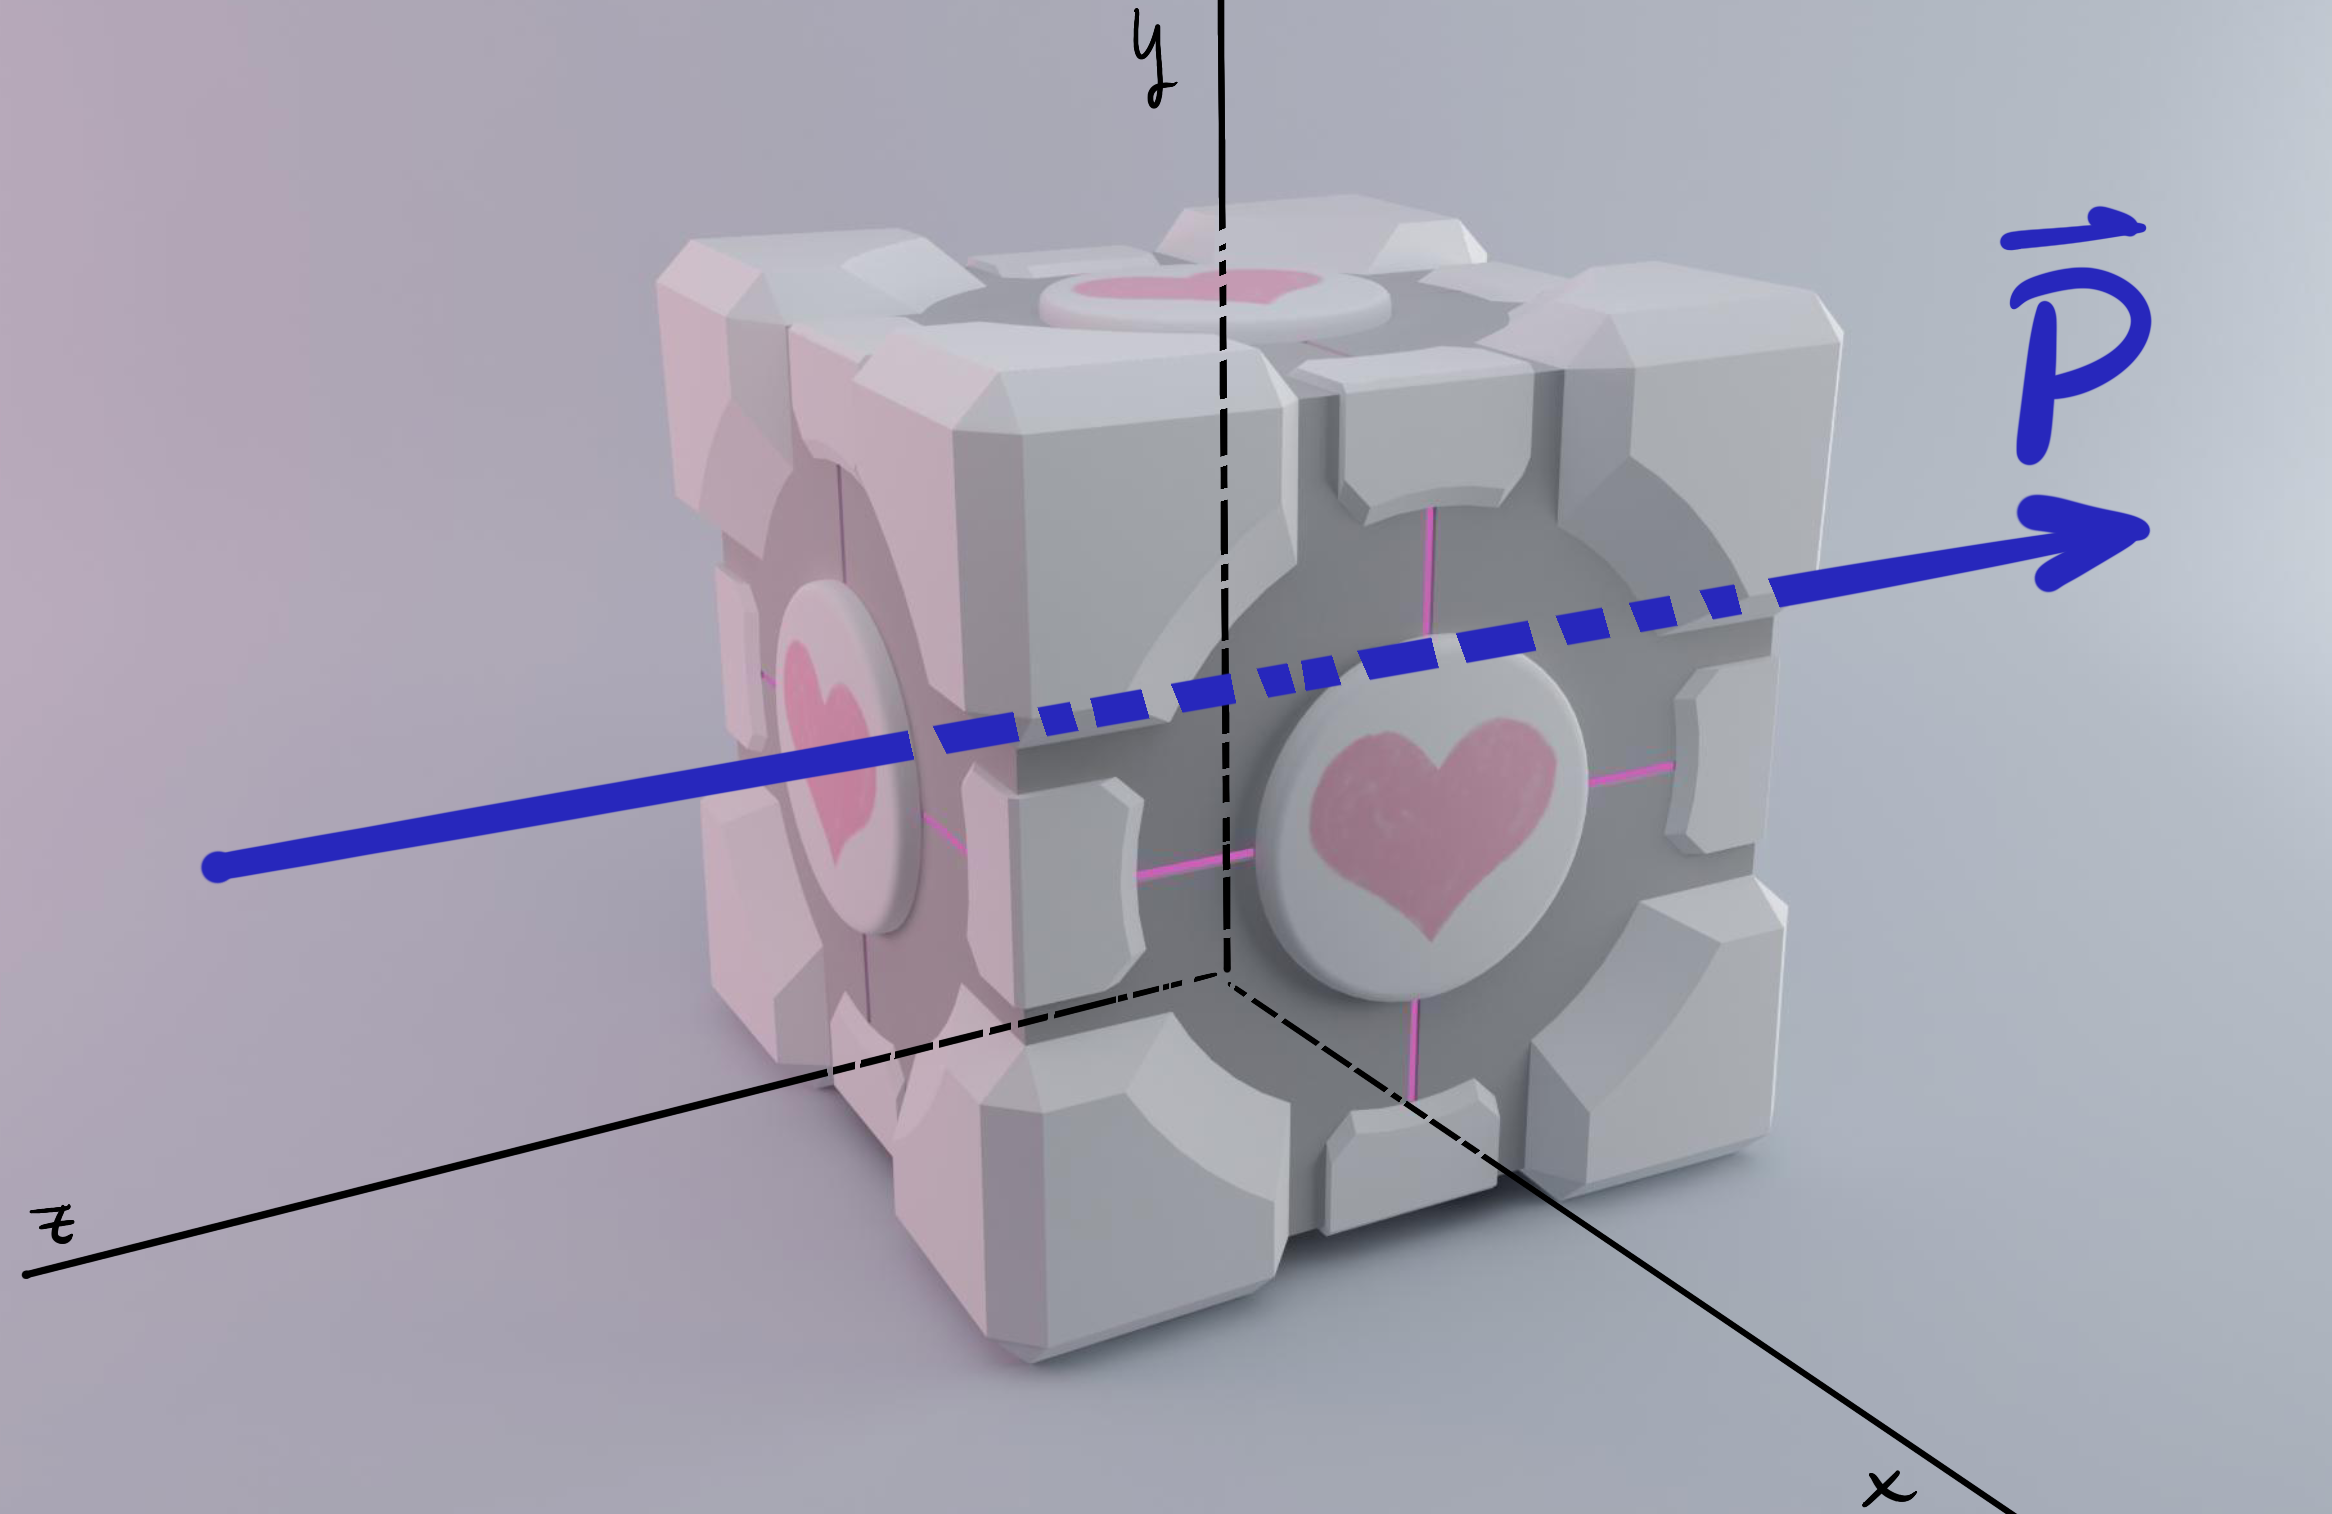
\includegraphics[width=8cm]{figures/Gladys.png}
	\centering
	\caption{But the cake is still a lie...}
\end{figure}

For this specific cubic case, we know that $\rho_{P}$ is 0, as our cube is homogeneously polarised, so $\mathbf{\nabla P} = 0$. The surface polarization $\sigma_{\mathbf{P}}=\mathbf{P} \cdot \hat{\mathbf{n}}$ is $P$ on the right $(R)$ face of the cube and $-P$ on the left $(L)$ face of the cube. Since we only have surface charge,

\begin{equation}
	\mathbf{E}(\mathbf{r})=\frac{P}{4 \pi \epsilon_{0}}\left[\int_{R} d S^{\prime} \frac{\mathbf{r}-\mathbf{r}^{\prime}}{\left|\mathbf{r}-\mathbf{r}^{\prime}\right|^{3}}-\int_{L} d S^{\prime} \frac{\mathbf{r}-\mathbf{r}^{\prime}}{\left|\mathbf{r}-\mathbf{r}^{\prime}\right|^{3}}\right].
\end{equation}

To simplify our lives, better to consider the value of all this when $\mathbf{r}=0$. Then, at the origin:

\begin{equation}
	\mathbf{E}(0)=-\frac{P}{4 \pi \epsilon_{0}}\left[\int_{R} d S^{\prime} \frac{\mathbf{r}^{\prime}}{r^{\prime 3}}-\int_{L} d S^{\prime} \frac{\mathbf{r}^{\prime}}{r^{\prime 3}}\right].
\end{equation}

By symmetry, the $x$ and $y$ components of these integrals are zero, as the polarisation only happens along the $z$-axis. Therefore, if the origin of the primed system is at the centre of the cube, we have:

\begin{equation}
	\begin{split}
		E_{z}(0) &=-\frac{P}{4 \pi \epsilon_{0}}\left[\int_{R} d S^{\prime} \frac{z^{\prime}}{r^{\prime 3}}-\int_{L} d S^{\prime} \frac{z^{\prime}}{r^{\prime 3}}\right]=-\frac{2 P}{4 \pi \epsilon_{0}} \int_{R} d S^{\prime} \frac{z^{\prime}}{r^{\prime 3}}= \\
		&=-\frac{2 P}{4 \pi \epsilon_{0}} \int_{R} d \mathbf{S}^{\prime} \cdot \frac{\mathbf{r}^{\prime}}{r^{\prime 3}}=\frac{2 P}{4 \pi \epsilon_{0}} \int_{R} d \Omega^{\prime} .
	\end{split}
\end{equation}

The integral is the solid angle subtended by the right face at the centre of the cube. By symmetry, this number must be $4 \pi / 6 .$ Therefore, the electric field at the centre of the cube is:

\begin{equation}
	\mathrm{E}(0)=-\frac{\mathrm{P}}{3 \epsilon_{0}}
\end{equation}

This is exactly the same as the electric field at the centre of a uniformly polarized sphere.


\subsubsection{E and D for an Annular Dielectric}\label{E and D for an Annular Dielectric}

\textbf{1):}

We are going to treat the geometry shown below as the superposition of a ball with radius $b$ and uniform polarization $\mathrm{P}$ and a concentric ball with radius $a$ and uniform polarization $-\mathrm{P}$.

\begin{figure}[h!]
	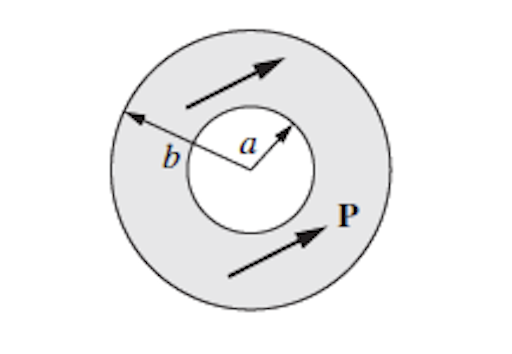
\includegraphics[width=8cm]{figures/PolarisatedBall.png}
	\centering
	\caption{The two concentric spheres and the polarisation $\mathbf{P}$.}
\end{figure}

From the text, the field produced by an origin-centered polarized ball with volume $V$ is:
	
\begin{equation}
	\mathbf{E}(\mathbf{r})=\left\{\begin{array}{ll}-\frac{\mathbf{P}}{3 \epsilon_{0}} & r<R \\
	\frac{V}{4 \pi \epsilon_{0}}\left\{\frac{3(\mathbf{r} \cdot \mathbf{P}) \mathbf{r}}{r^{5}}-\frac{\mathbf{P}}{r^{3}}\right\} & r>R
	\end{array}\right.
\end{equation}

Therefore, the field we want to study is given by:
\begin{equation}
	\mathbf{E}(\mathbf{r})=\left\{\begin{array}{ll}
		0 \quad & r<a, \\
		-\frac{\mathbf{P}}{3 \epsilon_{0}}-\frac{a^{3}}{3 \epsilon_{0}}\left\{\frac{3(\mathrm{r} \cdot \mathbf{P}) \mathbf{r}}{r^{5}}-\frac{\mathbf{P}}{r^{3}}\right\} & a<r<b, \\
		\frac{b^{3}-a^{3}}{3 \epsilon_{0}}\left\{\frac{3(\mathbf{r} \cdot \mathbf{P}) \mathbf{r}}{r^{5}}-\frac{\mathbf{P}}{r^{3}}\right\} & r>b
	\end{array}\right.
\end{equation}

\textbf{2):}

By symmetry, we should have $\mathbf{D}(\mathbf{r})=D(r) \hat{\mathbf{r}}$. Therefore, the choice of a spherical Gaussian surface of radius $r$ gives:

\begin{equation}
	\int_{S} d \mathbf{S} \cdot \mathbf{D}=D(r) 4 \pi r^{2}=Q_{c, \text{encl}}=0.
\end{equation}

Therefore, $\mathbf{D}=0$ everywhere.
	


\subsubsection{E: A Charge and A Conducting Sphere}\label{E: A Charge and A Conducting Sphere}
\textbf{\textcolor{red}{UNDER CONSTRUCTION}}

\subsubsection{E: Critical strain}\label{E: Critical strain}

\textbf{1):}

The capacitor system with two plates can vary its width, as the dielectric filling the space between the plates is elastic. If we want to find an equilibrium point, we need to compute the minima of stability of the potential controlling this system. In this case we will have two different potential energies: The electric one, stored inside the capacitor itself and the mechanical one, given by the elastic properties of the "spring" between the plates. The electromagnetic energy stored inside a capacitor is given by:\\
	
\begin{equation}
	U_{EM} = \frac{1}{2}\: A \: d \vec{E}\cdot \vec{D} = \frac{d \:q^{2}}{2 \:A \: \epsilon}.
\end{equation}

As the charge $q$ is constant at equilibrium, the equilibrium position $d(q)$ will be given by just the derivative of the total energy $U$ of the system derived respect to $d$, i.e.:

\begin{equation}
	U_{T} = U_{EM} + U_{\text{elas}} \rightarrow \partial_{d} U_{T} = 0, \rightarrow d = d_{0} - \frac{q^{2}}{2 A \epsilon k}.
\end{equation} 

\textbf{2):}

The potential inside a capacitor is given the norm of the electric field times the separation of plates, as:

\begin{equation}
	\Delta V = \|\vec{E}\| d = \frac{q\:d(q)}{A \epsilon} = \frac{q}{A \epsilon} \left(d_{0}- \frac{q^{2}}{2 A \epsilon k}\right).
\end{equation}

Observe that this expression has two roots: $q =0$ and $q = \sqrt{2 A \epsilon k d_{0}}$. It also has a maximum for $q$ lying at $q_{max} = \tfrac{\sqrt{3} \:q_{0}}{3}$. If we plot these results, we see that:
	
\begin{figure}[h!]
	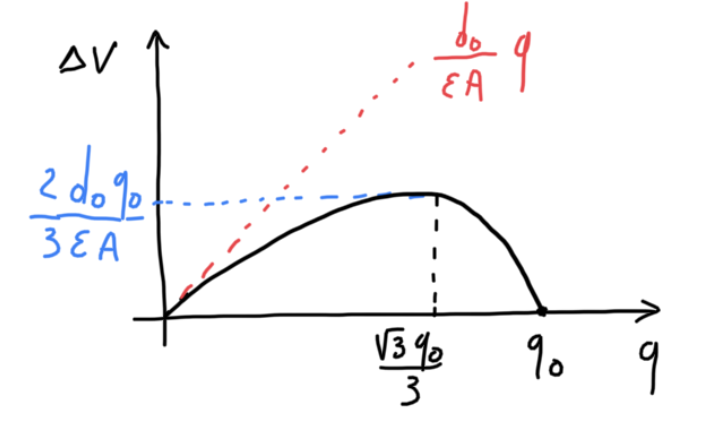
\includegraphics[width=5.1cm]{figures/PotentialConstraint.png}
	\centering
	\caption{The potential for this elastic capacitor.}
\end{figure}

At the critical point $q_{0}$, the whole capacitor collapses, pointing to the instability of this system.

